%%% Thesis chapter1 --------------------------------------------------
\chapter{Effect of Quantum Delocalization on Temperature 
Dependent Double Proton Transfer in Molecular Crystals of Terephthalic Acid } \label{chapter1}
%\footnotetext{Reprinted (adapted) with permission from \emph{Surface Science}, \textbf{2016}, 644, 69-79.}
\ifpdf
    \graphicspath{{Chapter1/Chapter1Figs/}}
\fi
 
% ------------------------------------------------------------------------
\section{Introduction}
\label{intro}

Multiple hydrogen/proton transfer (MPT) reactions play a crucial role in a variety of important processes. The replication of DNA, one of the most fundamental biological  processes, is prone to mutations,\cite{jacquemin2014assessing} which are created by complex steps involving MPTs. MPTs also have a prominent role in enzyme catalysis\cite{kirby1997efficiency,blomberg2006different,richard2012paradigm} as well as in other non-biological systems such as ionic liquids\cite{yoshizawa2003ionic} and organic solids\cite{horiuchi2008organic}. Moreover, the transfer of protons can also be coupled to changes in the underlying electronic structure of the system as seen in proton-coupled electron transfer reactions (PCET).\cite{huynh2007proton,costentin2010update,hammes2010theory,dempsey2010proton,warren2010thermochemistry} PCET reactions are ubiquitous and diverse. For example, excited state proton transfer\cite{arnaut1993excited,zhou2018unraveling}, has potential applications for use as a fluorescent probe\cite{sedgwick2018excited} in biological imaging\cite{yang2014macro} and also for use as an organic opto-electronic material\cite{kwon2011advanced}.

Majority of the MPTs are found in organic molecules like DNA base pairs\cite{watson1953molecular} and their analogues\cite{douhal1995femtosecond,ogawa2000phototautomerizable,abou2001tautomerization}, porphyrin\cite{storm1972nitrogen}, porphycene\cite{waluk2017spectroscopy}, phthalocyanines\cite{liljeroth2007current}, and carboxylic acids\cite{loerting1998toward} where the transfer of two protons generate tautomers. This special category of proton transfer induced tautomerization\cite{antonov2013tautomerism} is classified as double proton transfer (DPT). Depending on the manner in which the two hydrogen atom transfers, the overall process can have two mechanisms namely stepwise or concerted. Typically, a stepwise proton transfer involves individual hydrogen atoms/protons moving separately resulting in metastable intermediates. For example, Zewail and coworkers reported the hydrogen atoms of 7-azaindole dimers\cite{douhal1995femtosecond}, a prototypical system to the DNA base pair, transfer in a non-concerted manner generating ionic intermediate species. On the contrary, Kasha and coworkers\cite{catalan1999resolution} interpret the transfer of protons to have a concerted mechanism where the protons are transferred simultaneously resulting in a single non-ionic transition  state. The stepwise process involves charged intermediates and in most cases, have higher activation barriers whereas the concerted pathway suffers from the small kinetic pre-factor of two atoms transferring at the same time. The competition between the two processes determine the rate of tautomerization and the proportion of tautomers, which are essential in enzymatic reactions\cite{zhu2016tautomerization} and drug delivery\cite{wojnarowska2016tautomerism}.

Since hydrogen atoms are the lightest ones in the periodic table, their structural and dynamical properties are strongly influenced by nuclear quantum effects (NQE). NQEs in DPT processes are typically manifested through zero-point energy and tunnelling. While the zero-point energy fluctuations usually affect free energy barriers, tunnelling facilitates classically forbidden pathways at lower temperature. These manifestations in DPT are not only of fundamental interest in biological processes\cite{klinman} but are equally important in other chemical reactions\cite{nqerect, nqebio}. For example, Ivanov et al.\cite{ivanov2015quantum} and Wikfeldt et al.\cite{wikfeldt2014communication} used path integral molecular
dynamics (PIMD) simulations to capture NQEs in the dimer of formic acid and anti-ferroelectric squaric acid crystals respectively. They find the intermolecular DPT occurs through concerted proton transfer and is temperature dependent. Similarly, Cahlik et al.\cite{cahlik2021significance} using a combination of low temperature STM, atomic force microscopy (AFM) and PIMD simulations,  showed that the transferring hydrogen atoms in the one-dimensional quinonediimine molecular networks supported on Au(111) surface, are concerted. This promotes a delocalization of $\pi$-electrons along the molecular chain  providing enhanced mechanical stability and giving rise to new states in the gap. 
In the study on intramolcular DPT in a single molecule of porphycene,  Litman et al.\cite{porphycene_th} using PIMD simulations report the hydrogen atoms tunnel concertedly at low temperatures ($<$ 100 K) whereas a competition between the concerted and stepwise pathway is observed at high temperatures (100-300 K). Although these studies have provided novel and invaluable information regarding the nature of DPT, we note that most of these studies are primarily cases where the effect of crystal environment have been either ignored by taking single molecule and dimer or partially incorporated through a chain of molecules. However, a complete description of crystal field, much like solvent effects\cite{kwon2007double}, is necessary. One of the discernible effect of crystal field is the non-degeneracy of the tautomers caused due to the induced asymmetry of the potential energy surface.\cite{meier1982structure} The non-degeneracy manifests by modifying the rates of tautomerization which are critical in systems where the proton transfer processes are controlled by external stimuli such as electric field, light, heat, and stress\cite{wang2021stimuli}.

These fascinating reports prompted us to undertake a theoretical study on the nature of DPT. Therefore, in this work we investigate DPT in molecular crystals of terephthalic acid (TPA). The choice provides a more realistic and less complicated system to understand the nature of DPT and how it is modulated by the environment. TPA is also used as a commercial precursor in the polymer industry\cite{fadzil2014brief}. Moreover, the molecules of TPA are used as ligands\cite{decker2020mof,mateo2019long} for synthesizing metal-organic frameworks and supramolecular complexes catering to a wide range of applications.\cite{zhou2012introduction} More recently, Karothu and coworkers\cite{karothu2016shape} observed that the application of thermal/mechanical stimulus on the crystals of TPA results in a polymorphic phase transition\cite{karothu2016shape,ahmed2019shape}. This behaviour is referred to as thermosalient/mechanosalient effect and has important applications in the design of transducers. 

TPA exhibits three crystalline forms, namely, form I, II and III\cite{bailey1967crystal, sledz2001new} of which form I is found to be stable till 500 K\cite{sledz2001new}. When form I is heated from low temperature to room temperature, it is known to undergo a continuous order-disorder transition.\cite{fjaer1986order, fischer1986structure} From their neutron diffraction studies, Fischer and co-workers determined the onset of disorder in the H positions to be around 80 K.\cite{fischer1986structure} Their results were further corroborated by temperature dependent Raman studies by Fjaer and coworkers.\cite{fjaer1986order} The temperature dependence of the disorder is examined using solid state nuclear magnetic resonance  (SS-NMR)\cite{meier1986structure,meier1982structure}. The dipolar lineshapes and relaxation rate measurements find the proton to dynamically exchange in an asymmetric potential. The temperature dependence of relaxation rate at high temperature was explained using chemical kinetics whereas at low temperature, a quantum mechanical tunnelling model was needed. The proton transfer barriers at low (high) temperature were inferred as 8 (27) meV. Similar values of barriers were estimated by Meier and coworkers\cite{meier1983neutron} from their inelastic neutron scattering studies. The authors commented that the small value of activation barrier at low temperature could be the energy difference between the vibrational ZPE of the two minima and emphasized the need for further examination.

Using Born Oppenheimer Molecular dynamics (BOMD) simulations and Path Integral Molecular Dynamics (PIMD) simulations coupled to the Generalized Langevin Equation based thermostat (PIGLET) we have studied the temperature dependent behaviour of NQEs on the DPT in form I of TPA. Our findings show that NQEs involve a tunnelling DPT mechanism at low temperatures ($<$ 100 K) whereas at room temperature (300 K), it is the zero-point energy fluctuations that increases the shuttling process by decreasing the activation barrier. Moreover, we observed that the DPT is concerted throughout the temperature range (70-300 K) where, as expected, the hydrogen atom shuttles like a proton. The rest of the chapter is divided as follows: in Section~\ref{compdet} we provide the details of the BOMD and PIMD simulations. The results are presented and discussed in Section~\ref{results}. Finally, we conclude in Section~\ref{concl} with some outlook and perspectives.


\section{Computational details}
\label{compdet}

Since form I is a stable polymorph of TPA between 70 and
300 K,\cite{sledz2001new, bailey1967crystal} the
temperature range of interest in this study, we have restricted our calculations
to form I. The crystal structure of this form was taken from the Cambridge 
Crystallographic Data Centre under the deposition number 1269122 and is optimized 
using the Broyden–Fletcher–Goldfarb–Shanno\cite{fletcher2013practical} (BFGS) algorithm where the electronic structure was calculated using the
Quickstep\cite{vandevondele2005quickstep} module, which is a Gaussian and Plane 
wave (GPW) based implementation of Density Functional Theory, in the open source 
CP2K\cite{hutter2014cp2k} package. The electronic exchange and correlation are
approximated within the generalized gradient approximation (GGA) framework proposed by 
Becke-Lee-Yang-Parr\cite{becke1988density,lee1988development} (BLYP). van der Waals 
interactions have been included using the Grimme's D3 
dispersion correction\cite{grimme2010consistent}. The electron-ion  
interactions were described by the norm-conserving, separable, dual-space 
Gaussian-type pseudopotentials of Goedecker, Teter, and 
Hutter\cite{goedecker1996separable} (GTH). The triple-zeta valence polarisation
(TZVP) basis set was used to expand the electronic wavefunctions. The 
charge density was expanded on a grid with a plane wave cutoff of 450 Ry. The 
electronic calculations were done using a 2$\times$2$\times$5 supercell. Brillouin zone integrations have been performed using only the $\Gamma$-point.

 
The BOMD simulations of TPA crystals were performed at 70, 100, 200 and 300 K
using a canonical sampling through velocity rescaling\cite{bussi2007canonical}(CSVR) 
thermostat as implemented in the CP2K package.
In order to study the effect of NQE, we have performed PIMD simulations at the same
temperatures. These simulations were carried out using the 
i-PI\cite{kapil2019pi} and CP2K software, where i-PI propagates the nuclear motion 
and CP2K calculates the electronic forces and energy. A coloured noise Generalised 
Langevin Equation based thermostat (GLE) is coupled to PIMD 
simulation\cite{ceriotti2012efficient} (PIGLET) to accelerate the convergence 
with respect to the number of beads. The converged number of beads for the 
PIGLET simulation at 70 K was estimated to be 16 (the results of the convergence tests are shown in 
Section \ref{convergence_si} of the Appendix \ref{appendix4}). For the higher temperature simulations we have used, for consistency, the same number of beads. The parameters for the diffusion and drift matrices of the coloured noise thermostat were generated from the online repository (\emph{http://gle4md.org/}) such that the maximum physical frequency lie close to 4000 cm$^{-1}$ for all
temperatures. The equations of motion in the various molecular dynamics simulations were integrated with a time step of 0.5 fs. The BOMD and PIGLET simulations were performed for 35 ps and 20 ps respectively. The analysis were done using the last 30 ps and 18 ps
of the BOMD and PIGLET trajectories respectively.
 
\section{Results}
\label{results}

\subsection{Crystal Structure of TPA}

Each TPA molecule consists of a benzene ring with two carboxyl group at each of
the para positions of the benzene ring (Figure \ref{fig:str_ptc}(a)). In the crystalline form, the 
molecules are arranged in chains that are formed through double hydrogen bonding
between the hydroxyl OH groups of the -COOH group of one TPA unit with the oxygen of the -COOH group in the 
neighbouring TPA unit. Two such chains are further bound together by weak H 
bonds between the H atoms of the phenyl group and the O atoms of the -COOH group
to give rise to a two-dimensional sheet. These two-dimensional sheets are
stacked on top of each other to give rise to the three-dimensional crystal
structure. Depending upon how two such
sheets are stacked, TPA exists in three polymorphs, namely form I, II and III, where, in case of the most stable form I (see Section \ref{form-si} of the Appendix \ref{appendix4} ), the TPA molecules of one sheet are on top of those
in the sheet below it, as shown in Figure~\ref{fig:str_ptc}(a). 

At 0K, the TPA molecules in form I are in the trans configuration (Figure~\ref{fig:str_ptc}(a)). This is also known as the L-tautomer.
When all the protons of the L-tautomer are transferred to the acceptor O atoms,
another configuration, namely the R-tautomer, can be formed
(Figure~\ref{fig:str_ptc}(b)). Both the tautomers crystallize in the triclinic form with the chain axis parallel to the $a$ lattice vector.
The former is about 19 meV/TPA molecule lower in energy than the latter.
For both the tautomers we obtain the same lattice parameters
($a$, $b$ and $c$ of 9.62, 7.61 and 3.62 \AA~respectively and
$\alpha$, $\beta$ and $\gamma$ of 73.80, 105.07 and 139.44$^{\circ}$
respectively). The lattice parameters obtained from our calculations
are given in Table \ref{tab:0K_str} of the Appendix \ref{appendix4} showing consistency with previous reports\cite{bailey1967crystal,sledz2001new}.

\begin{figure}
    \centering
    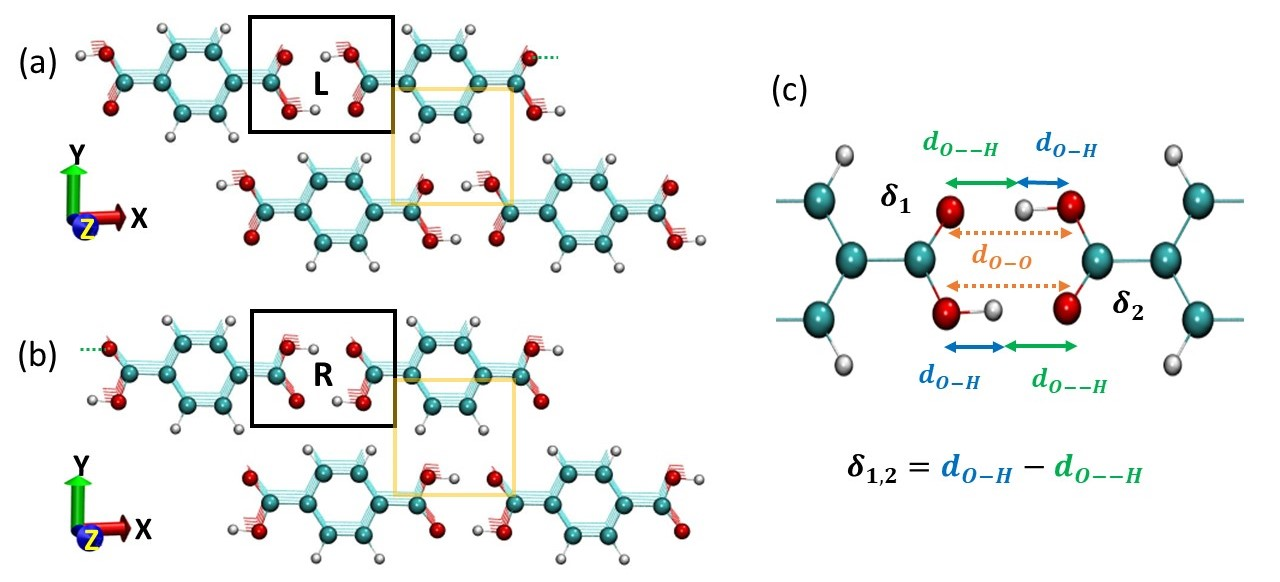
\includegraphics[width=16cm ]{./Chapter1/new_figures/structure_ptc.jpg}
    \caption{Crystal structure of form I of TPA using ball and stick 
    representation. Top view showing the stacking of the TPA chains in
    (a) L-tautomer and (b) R-tautomer. The red (yellow) square highlights the strong (weak) inter-molecular H-bonds that result in the formation of the chains (sheets).
    (c) The proton transfer coordinates
    $\delta_1$ and $\delta_2$ at a junction of two TPA molecules. In (a)
    and (b) the topmost layer atoms are shown with solid spheres and the bottom 
    layer atoms are shown as points. In this and the subsequent figures green, red and white spheres represent carbon, oxygen and hydrogen atoms respectively.}
    \label{fig:str_ptc}
\end{figure}

The TPA tautomers have two types of local interactions, (i) a pair of O-H$\cdots$O bond parallel to the chain direction (highlighted by a black square in Figure~\ref{fig:str_ptc}(a) and (b)), with a shorter heavy atoms separation of 2.63 \AA~in both the tautomers and (ii) a pair of C-H$\cdots$O bonds\cite{gu1999fundamental} perpendicular to the chain direction (highlighted by a yellow square in Figure~\ref{fig:str_ptc}(a) and (b)) with heavy atoms separation ($d_{C\cdots O}$) of 3.36 \AA{}  and 3.46 \AA{} in the L-tautomer where the shorter (longer) heavy atom separation is due to the interaction of the benzene hydrogen with the lone pair of the more (less) acidic \textit{sp$^3$} (\textit{sp$^2$}) hybridized carboxyl oxygen. The corresponding $d_{C\cdots O}$ in the R-tautomer are 3.42 \AA{} (where O is \textit{sp$^2$} hybridized) and 3.38 \AA{} (where O is \textit{sp$^3$} hybridized). On the basis of the heavy atom separation\cite{arunan2011definition,desiraju2001weak}, the O-H$\cdots$O is categorised as a strong hydrogen bond (sHB) whereas the C-H$\cdots$O falls under the category of \emph{improper} hydrogen bond. The \emph{improper\cite{van2001nature}} hydrogen bond are weak (wHB) hydrogen bonds which causes blue shift in the covalent bond ($C-H$) stretching. The dissimilar pairs of C-H$\cdots$O wHBs for the L and R-tautomer is responsible for lifting the degeneracy between the two tautomers. As a result, the associated DPT process occurs through a asymmetric double well potential which is discussed in Section \ref{whb-td} of the Appendix \ref{appendix4}.


\subsection{Finite Temperature NQE on strong hydrogen bonds} 

In order to analyze the proton transfer events, we define the following proton transfer coordinates ($\delta_{1,2}$) as shown in Figure \ref{fig:str_ptc}(c), where $\delta_{1,2}$ is the difference
between H-bond length between the acceptor oxygen atom and the transferring hydrogen atom ($d_{O\cdots H}$) and the covalent bond length between the donor oxygen atom and the same transferring hydrogen atom ($d_{O-H}$). At 0 K, in the L-tautomer of form I, the protons are bonded to the donor oxygen atoms and exhibits the ordered state resulting in a negative value of $\delta_{1,2}$. Fluctuations of the $\delta_{1,2}$ between positive and negative values indicate the occurrence of proton transfer events. 


\noindent \textit{Stepwise versus concerted DPT.} The dependency between $\delta_{1}$ and $\delta_{2}$ provides insight into the underlying DPT process. Therefore, in order to understand the the DPT mechanism (stepwise or concerted) and the temperature dependence of NQEs, we have plotted the effective free energy ($F_{eff}$) corresponding to the joint  probability distribution function (JPDF) between the $\delta_1$ and $\delta_2$ (Figure~\ref{fig:delta1_delta2}) at 70 and 300 K for the BOMD and PIGLET simulations. The free energy ($F$) corresponding to a discrete and normalized JPDF ($p$) between two quantities $X$ and $Y$ at ($X_i$, $Y_j$) can be written as: 

\begin{equation}
   F(X_i,Y_j) = -k_{B}T \; ln[\;p(X_i,Y_j) \; dX\;dY] 
    \label{free_energy}
\end{equation}

\noindent where $k_B$ and $T$ are the Boltzmann constant and the simulation temperature, respectively. $p(X_i,Y_i)$ is the normalized JPDF of $X$ and $Y$ at $X_i$ and $Y_j$ respectively. $dX$ and $dY$ are the binning widths used to discretize the $X$ and $Y$ variables respectively. The minima of the discrete free energy surface correspond to the maxima of the joint probability. The effective free energy ($F_{eff}(X_i,Y_j)$) is computed by shifting all $F(X_i,Y_j)$ with the $F^{min}(X_{min},Y_{min})$ as shown in the 
equation below:

\begin{equation}
 \label{free_energy_eff}
 F_{eff}(X_i,Y_j) = F(X_i,Y_j) - F^{min}(X_{min},Y_{min})
\end{equation}

Stepwise proton transfer events will result in local minima in the free energy plots at all the four quadrants since sequential transfers, in addition to the two tautomers at the first and third quadrants, will also generate the (two) ionic intermediates at the second and fourth quadrants. At 70 K, for the classical nuclei,
since there are no proton transfer events, we observe a single local minima
in the third quadrant (Figure~\ref{fig:delta1_delta2}(a)).
Upon increasing the temperature to 300 K, we find minima in both the 
first and third quadrant (Figure~\ref{fig:delta1_delta2}(b)) showing that finite temperature induces concerted proton transfer events.

When the NQE are turned on, local minima of FES are observed in the first and third 
quadrant even at 70 K (Figure~\ref{fig:delta1_delta2}(c)). This of course implies that the proton is significantly more delocalized along the hydrogen bonds fully consistent with previous studies reporting this effect in numerous other organic molecular systems\cite{fang2016inverse,li2011quantum,wang2014quantum,ivanov2015quantum,wikfeldt2014communication,litman2019elucidating,sappati2016nuclear,rossi2016anharmonic,pinotsi2016proton,law2015role,tuckerman1997quantum}. Furthermore, the free energy profile extends to the second and 
fourth quadrant forming an \emph{elbow} suggesting that there are events where both the transferring 
protons are on the same molecule. We note that the presence of such configurations
are indications of occurrence of step-wise proton transfers. However,
since these are higher in energy, their occurrences are rare. Further,
we did not observe any local minima in the \emph{elbow} regions of the free energy profile, which would be
characteristic of step-wise proton transfer. All in all, these results suggest that the DPT in the TPA crystal is primarily a concerted process.

\begin{figure}
\centering
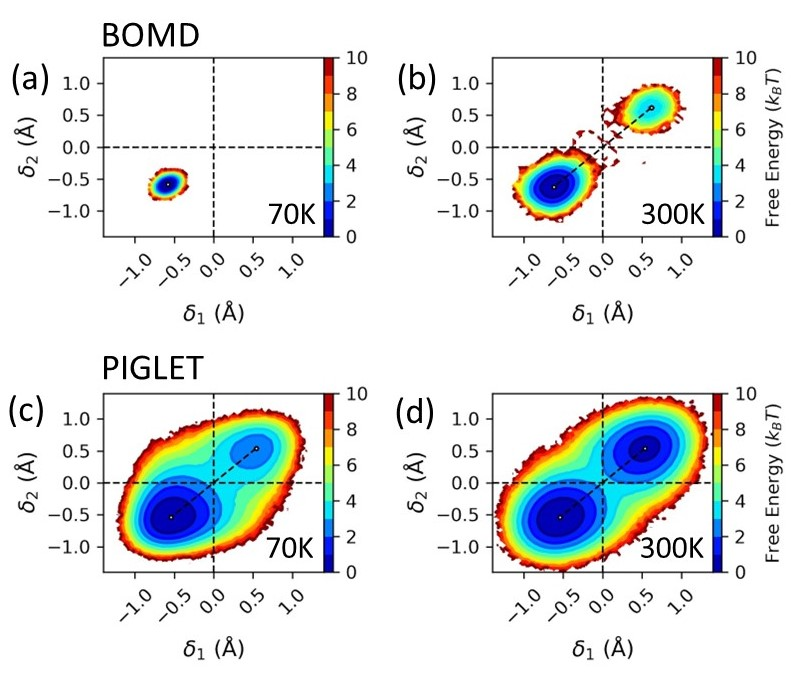
\includegraphics[width=14cm ]{./Chapter1/new_figures/prob_delta1_delta2.jpg}
\caption{The effective free energy ($F_{eff}$) as a function of the proton transfer
coordinates $\delta_1$ and $\delta_2$ at
70 (left column) and 300 K (right column). The top and bottom row are
from BOMD and PIGLET simulations respectively.}
\label{fig:delta1_delta2}
\end{figure}

Upon increasing the temperature to 300 K, we find an enhanced proportion of events in the first quadrant suggesting an increase in proton transfer activities. This symmetrizes the shape of the FES in the first and the third quadrant indicating that at this temperature the disorder in the hydrogen bond network is almost complete. Additionally, the spread of the free energy profile decreases (the \emph{elbow} observed at 70 K softens) along the $\delta_1 = -\delta_2$ direction. This implies that at higher temperatures the probability of finding the configurations where both the protons are on the same molecule is diminished. This behaviour is linked to the loss of correlation between the two transferring protons due to quantum tunneling at 70 K and is discussed in section \ref{losss} of the appendix \ref{appendix4}.
 

\noindent \textit{Quantum tunnelling versus activated hopping.} Our simulations also allow for disentangling the relative role of quantum tunnelling vs activated proton hopping driven by zero point energy fluctuations. The relative role of these two effects will naturally be temperature dependent. The effect of quantum tunnelling can be quantified by an increase in the radius of gyration of the ring polymer representing the quantum nucleus\cite{ceriotti_hbond_fluc}. The radius of gyration probes the quantum uncertainty in position of the nucleus and is proportional to the thermal de Broglie
wavelength of that nucleus. Hence, it is expected that a proton transfer
event due to tunnelling is to be accompanied with an enhancement of the radius of gyration of the proton. Therefore, to examine the extent of this effect, we have computed the radius of gyration, $r_G = 
\sqrt{\frac{1}{P}\sum_{i=1}^{P} (\mathbf{r_i^H}-\mathbf{r_c^H})^2}$,  where H is the hydrogen atom,
$P$ is the number of beads in the ring polymer, $\mathbf{r_i^H}$ is the position of the H-atom in the $i^{th}$ 
bead of the proton ring polymer and $\mathbf{r_c^H}$ is the position of the centroid of the proton ring polymer 
($\mathbf{r_c^H}=\frac{1}{P}\sum_{i=1}^{P} (\mathbf{r_i^H)}$).

Figure~\ref{fig:tunnel2}(a) and (b) shows the proton 
transfer coordinate of the centroid of the ring polymer ($\delta_o^C$; blue graph) and its radius of gyration  ($r_G$; red graph) as a function of the simulation time at 70 and 300 K.
We note that at 70 K, whenever $\delta_0^C$ changes sign there is a peak/enhancement of $r_G$ (Figure~\ref{fig:tunnel2}(a)) suggesting that the quantum fluctuations is
delocalizing the proton that is being transferred thereby resulting in an
enhancement of its de Broglie's wavelength, a consequence of which is that the
proton is tunnelled from one potential well to another. In contrast,
at T=300 K (Figure~\ref{fig:tunnel2}(b)), we do not observe any 
enhancement of $r_G$ when a proton transfer event is occurring suggesting
that for this case, the proton transfer is activated hopping from one minima to another.

\begin{figure}
\centering
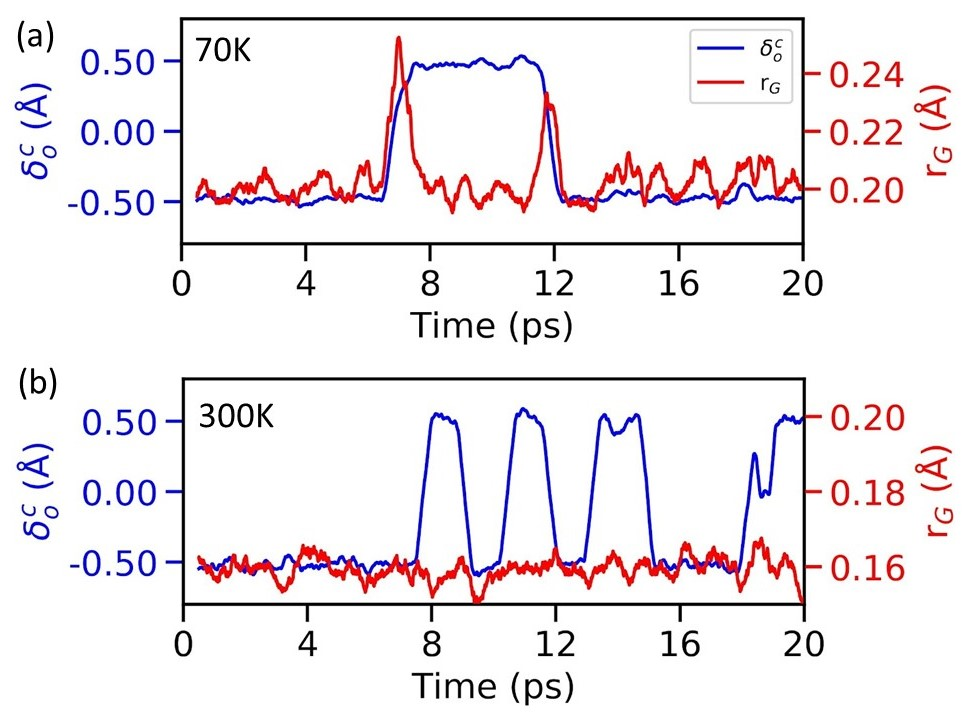
\includegraphics[width=15cm ]{./Chapter1/new_figures/tunnelling_vs_shuttling_2.jpg}
\caption{Plots of $\delta_o^C$ and $r_G$ as a function of sampling time
at (a) 70 and (b) 300 K. }
\label{fig:tunnel2}
\end{figure}

\begin{figure}
\centering
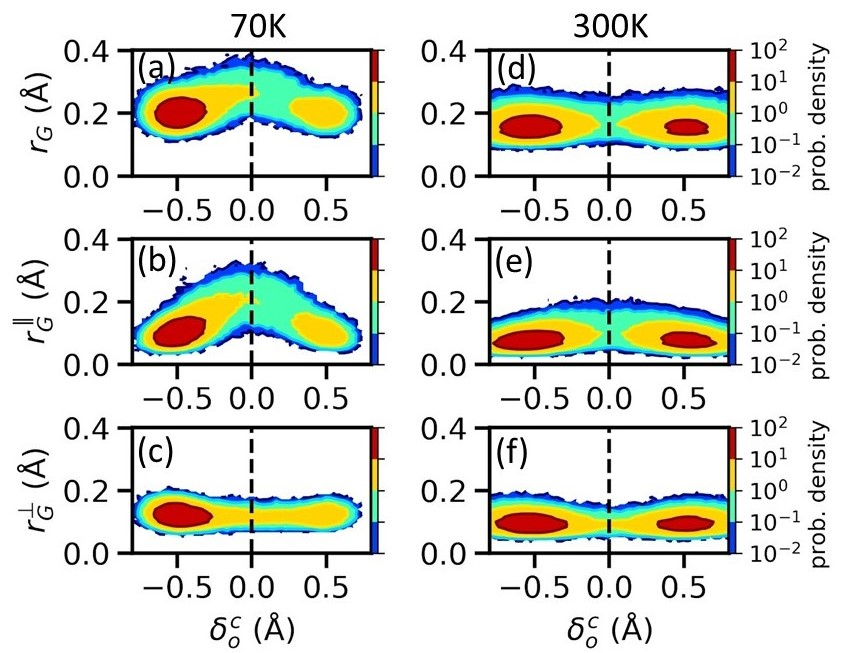
\includegraphics[width=15cm ]{./Chapter1/new_figures/tunnelling_vs_shuttling_1.jpg}
\caption{The joint density plots of $\delta_o^C$ and radius of gyration at 70 K (left panel) and 300 K (right panel). (a) and (d) correspond to the radius of gyration ($r_G$), (b) and (e) correspond to the component of $r_G$ parallel to the O-H bond ($r_G^{\parallel}$), and (c) and (f) correspond to the component of $r_G$ perpendicular to the O-H bond ($r_G^{\bot}$).}
\label{fig:tunnel1}
\end{figure}

For further confirmation of the relative role of tunnelling versus zero-point energy 
fluctuations in DPT, we constructed the joint probability distributions of $r_G$ 
and $\delta_0^C$
(Figure~\ref{fig:tunnel1}(a) and (d) at 70 and 300 K respectively).
If the proton transfer occurs due to tunnelling, we expect a large spread in 
$r_G$ at around $\delta_0 = 0.00$. Additionally, this delocalization should be
along the direction of the H-bond for the tunnelling to occur from one well
to the other. To check whether this is indeed the case for our system, we have also
computed the projection of $r_G$ on the parallel ($r_G^{\parallel}$,
Figure~\ref{fig:tunnel1}(b) and (e) at 70 and 
300 K respectively) and perpendicular directions ($r_G^{\perp}$, Figure~\ref{fig:tunnel1}(c) and (f) at 70 and 
300 K respectively) of the hydrogen bond.
Consistent with our previous observation for a single proton transfer coordinate, here also we find that
at T=70 K, there is a large spread of $r_G$ at around $\delta_0$=0.00 
(Figure~\ref{fig:tunnel1}(a)) while the spread is uniform for T=300 K (Figure~\ref{fig:tunnel1}(d)). Analysing the
contributions from the parallel and perpendicular components of $r_G$, we note that these
enhancements at 70 K are due to enhancements observed in $r_G^{\parallel}$
(Figures~\ref{fig:tunnel1}(b) and (e)), 
thereby further verifying that at 70 K, the proton transfer occurs through
tunnelling while at 300 K it is due to activated hopping. Similar analysis at
different temperatures (Figure \ref{fig:cip11}, in the Appendix \ref{appendix4}) show that the transition from tunnelling to complete hopping occurs at around 200 K.


\noindent \textit{Correlation between proton transfer and H-bond fluctuations} The manifestation of NQEs in these type of systems are not restricted to the distribution of the transferring protons but also affect the vibrations of the 
heavy atoms connected to the proton transfer coordinate. The vibronic coupling of the heavy atoms with the protons is prominent in most hydrogen bonded 
systems such as protonated  water\cite{marx1999nature, hassanali2013proton, benoit2005shapes}, protein analogues\cite{zhou2020symmetry}, crystal 
hydrates\cite{hassanali2012fuzzy,buch2007elusive,buch2008hcl} and even other molecular crystals\cite{wikfeldt2014communication,srinivasan2011isotope}. Using PI simulations on a 
single Zundel ion, Benoit et al.\cite{benoit2005shapes} reported the dependence of the proton transfer on the distance between the oxygen atoms. A large 
separation leads to the proton being localized on one water separated by a large barrier. On reducing the separation to ultra small values, the two peaks 
merge into one broad peak corresponding to a single potential well. Similar effects have also been observed in molecular dynamics simulations of various 
crystal hydrates\cite{hassanali2012fuzzy,buch2007elusive,buch2008hcl}.

This dependence in TPA is illustrated by computing the joint probability
distribution as a function of the proton
transfer coordinate ($\delta_{1,2}$) and its heavy atom separation ($d_{O-O}$), resulting in \emph{banana-shaped} free energy profiles
(Figure \ref{fig:delta_OO}). Careful inspection of the free
energy profiles obtained from the BOMD simulations at 70 and 300 K
((Figure~\ref{fig:delta_OO}(a) and (b), respectively) shows that the proton transfer is coupled to a mild reduction in the $d_{O-O}$.
At both the temperatures (70 and 300 K) we obtain a linear correlation with Pearson correlation coefficient between $\delta_{1,2}$ and
$d_{O-O}$ of $\pm 0.83$ for positive and negative
values of $\delta_{1,2}$. 


\begin{figure}
\centering
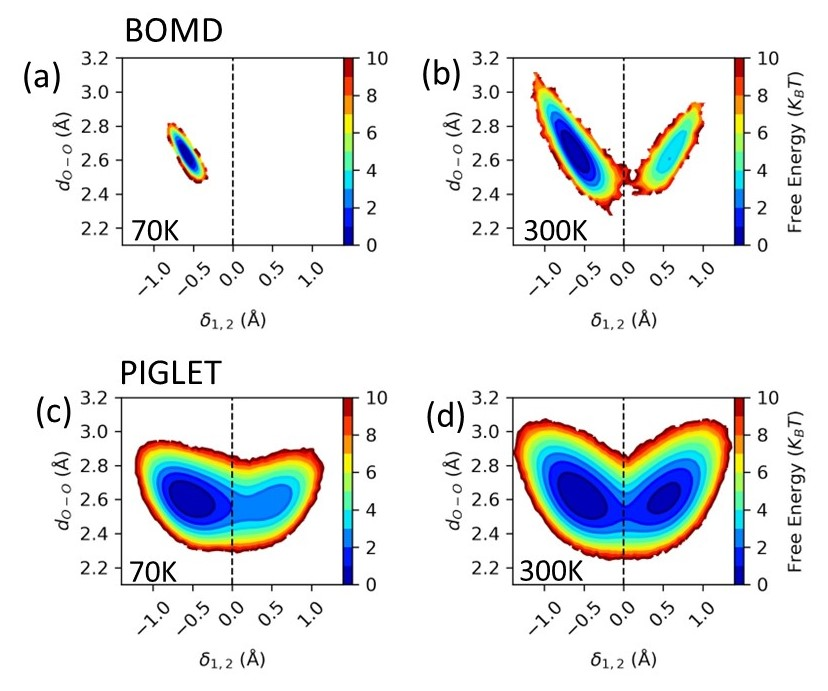
\includegraphics[width=16cm ]{./Chapter1/new_figures/prob_delta_OO.jpg} 
\caption{The effective free energy as a function of the proton transfer
coordinate ($\delta_{1,2}$) and the heavy atom distance ($d_{O-O}$) at
70 (left column) and 300 K (right column). The top and bottom row are
from BOMD and PIGLET simulations respectively.}
\label{fig:delta_OO}
\end{figure}

Upon turning on the NQE, we observe an asymmetric \emph{banana-shaped} free energy profile, even at 70 K (Figure~\ref{fig:delta_OO}(c)), with two minima, one at $\delta=-0.54$ \AA{}, $d_{O-O}=2.61$ \AA{} and the other at 
$\delta$ = 0.5 \AA{}, $d_{O-O}$ = 2.58 \AA{}, suggesting that proton transfer events occur at low temperatures.
Moreover, for both the negative and positive values of $\delta_{1,2}$ we observe a larger
spread along the $d_{O-O}$ axis suggesting a weakening of the coupling between the shrinkage of
the O-O distance and proton transfer compared to that observed when NQEs are ignored.
Indeed the Pearson correlation coefficient is reduced to -0.39 for $\delta_{1,2}$ $<$ 0 and 0.38 for $\delta_{1,2}$ $>$ 0 at 70 K. Increasing the temperature to 300 K, we observe that the spread of the free energy profile increases (Figure~\ref{fig:delta_OO}(d)). However, the Pearson correlation coefficients are improved (-0.53 for $\delta_{1,2} < 0$ and 0.54 for $\delta_{1,2} > 0$) compared to that observed at 70 K from PIGLET simulations. These results suggest that while NQE weakens the coupling between proton transfer and the shrinkage of the O-O distance, the latter is enhanced with increase in temperature.

We further note that occurrence of proton transfer events at 70 K is in accordance with the experimental observations where the order disorder transition sets in at around 80 K.\cite{fjaer1986order, fischer1986structure} The free energy
difference between the two minima is about 13 meV. The asymmetric nature of the FES, as discussed earlier, can be attributed to the crystal field effect where the L and R tautomers are not degenerate. At 300 K the difference between these two minima increases marginally to 15 meV. Moreover, a comparison of the heavy atom distances, $d_{O-O}$ between BOMD ( 2.63 \AA {} at 70 K and 2.65 \AA{} at 300 K) and PIGLET (2.60 \AA{} at 70 K and 2.62 \AA{} at 300 K) shows that the NQEs strengthen the strong H-bonds. We note that similar strengthening has been observed in pentamers and hexamers of HF\cite{li2011quantum}, charged clusters of N$_2$H$_5^{-}$\cite{li2011quantum}, dimers of formic acid\cite{li2011quantum}, a molecular chain of 2,5-diamino-1,4-benzoquinonediimine\cite{cahlik2021significance} on Au(111) and solid HF and squaric acid\cite{wikfeldt2014communication,li2011quantum}.


\subsection{Charge state of the transferring H atom} 

The shuttling of the H atom involves simultaneous cleavage and formation of 
covalent O-H bonds. Intuitively, one might expect that during the proton 
transfer event the H atom is transferred as H$^+$, particularly when it is 
equally shared between donor and acceptor oxygen atoms. To 
verify this and to understand the effect of the proton transfer fluctuations on 
the electronic density, we have computed the maximally localized Wannier 
functions (MLWF)\cite{marzari1997maximally,marzari2012maximally}. A single 
Wannier center can be associated with an electron pair.
Each O atom of the -COOH group of TPA is associated with four Wannier centres.
At 0 K, the Wannier centre corresponding to the covalent O$_{donor}$-H bond
is 0.55 \AA~away from the H atom. On the other hand the acceptor O 
atom that forms the C$=$O bond has a pair of Wannier centres at about 
0.32 and 0.35 \AA~corresponding to the lone pairs. As the proton moves from
the donor O to the acceptor O, we monitored the change in the distance between (i) the position of the Wannier centre between the donor O (of the -OH covalent bond)
and H atom (labelled as $d_{X'-H}$ in Figure \ref{fig:wannier}(a)) and (ii)
the position of the Wannier centre of the lone pair of the acceptor O atom 
(forming C$=$O bond) directed along the H-bond (labelled as $d_{X''-H}$ in 
Figure~\ref{fig:wannier}(a)). 

\begin{figure}
\centering
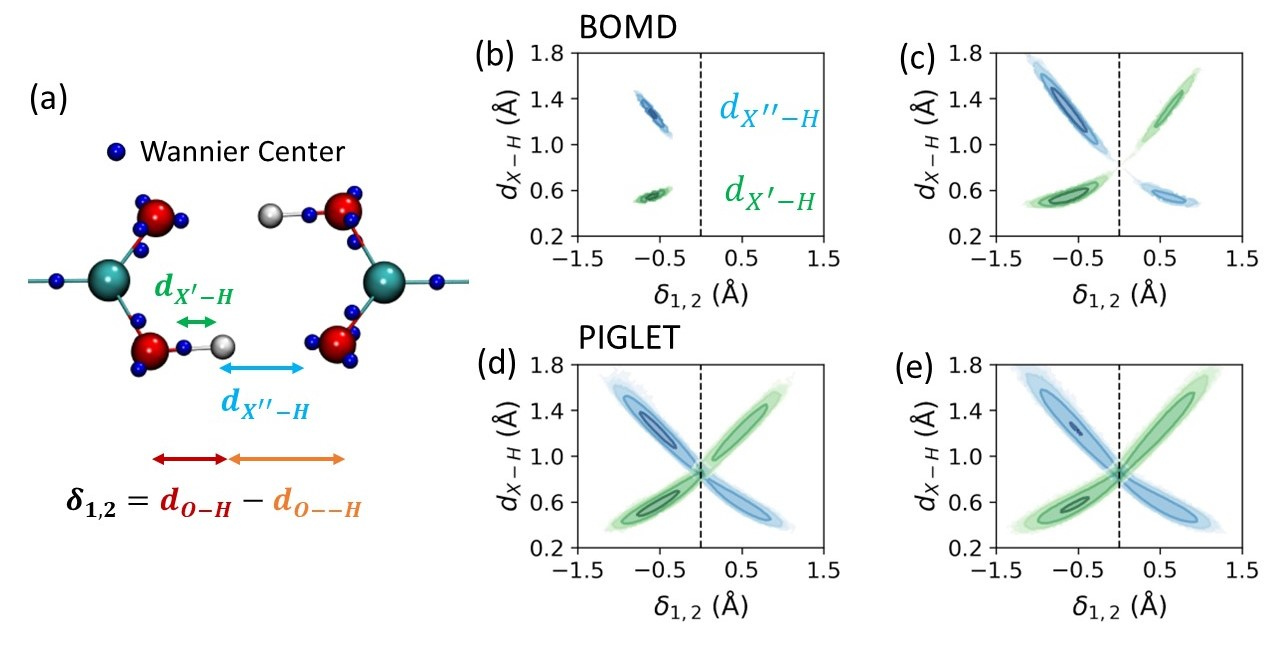
\includegraphics[width=15cm ]{./Chapter1/new_figures/wannier.jpg}
\caption{ (a) The positions of the O Wannier centres denoted by blue spheres. The distance, $d_{X'-H}$, between O (donor)-H Wannier center from the H and $d_{X''-H}$, between the H and the nearest Wannier center corresponding to one of the two lone pairs at the acceptor O are also marked. (b)-(d): The joint probability distribution between the two distances ($d_{X'-H}$ and $d_{X''-H}$) and proton transfer coordinate obtained from BOMD (top panel) and PIGLET (bottom panel) simulations at 70 K (left column) and 300 K (right column).}
\label{fig:wannier}
\end{figure}

Figure~\ref{fig:wannier}(b) and (c) (Figure~\ref{fig:wannier}(d) and (e))
show the joint probability distribution 
plots of $d_{X'-H}$ and $d_{X''-H}$ with $\delta_{1,2}$ for the BOMD (PIGLET) 
simulations at 70 and 300 K, respectively. For the BOMD simulations at 70 K where no proton transfer events was observed, the position of the Wannier centres
fluctuate about their mean position and are localized.  When the temperature is raised to 300 K, the fluctuations increase and only for those cases where the proton transfers occur the $d_{X'-H}$ and $d_{X''-H}$ switch their values
suggesting that the Wannier centre of the donor O atom moves closer to it
and that of the acceptor O moves away from it. 
 

However, on turning on the NQE we notice
that there is a non-zero probability when $d_{X'-H} = d_{X''-H}$. This implies that the Wannier centre
corresponding to the covalent O-H bond moves closer to the O atom resulting in a charge
transfer to the donor O atom. Upon monitoring the evolution of the two Wannier
functions during the proton transfer path, we observe that when the H-atom
is covalently bonded to one of the O-atoms (forming L or R-tautomer),
the Wannier functions, as expected, are similar to that of an -OH bond and an O-lone pair (Figure~\ref{fig:wannierII}(a) and (c) for L and R tautomers respectively). However, when the proton is shared equally between the two H atoms, the Wannier functions of the donor and acceptor O atoms are similar to that of an O-lone pair
(Figure~\ref{fig:wannierII}(b)) suggesting that the electron pair
involved in forming the covalent -OH bond is localized on the donor
O atom. As a consequence, the shuttling H atom shared between
the two O atoms behaves as a proton. We would like to emphasise that this is a purely quantum effect of the delocalization of the H nuclei and is not observed in the BOMD simulations where the nuclei are treated classically.

\begin{figure}
\centering
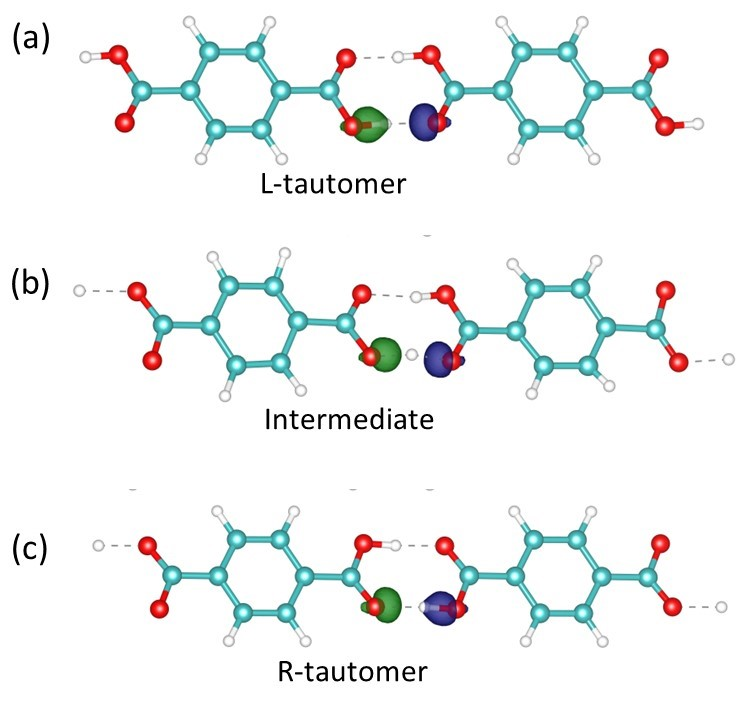
\includegraphics[width=10cm ]{./Chapter1/new_figures/function_wann.jpg}
\caption{Evolution of the Wannier functions of the O$_{donor}$-H bond (green 
isosurface) and the O$_{acceptor}$ lone pair (blue isosurface) as the proton
transfers from the donor to the acceptor oxygen. (a) H covalently bonded to 
donor O forming L-tautomer, (b) the H atom is equally shared by the donor and 
acceptor and (c) the H atom covalently bonded to acceptor O atom, R-tautomer. For
clarity, only a pair of TPA molecules where the proton transfer is occurring is 
shown.}
\label{fig:wannierII}
\end{figure}


\section{Summary and Conclusions}
\label{concl}

In summary, using the state of the art PIGLET simulations, we have studied
temperature dependent double proton transfer in molecular crystals of
terephthalic acid. In accordance
with experiments, we observe occurrence of proton transfers and thereby
onset of order-disorder transitions at temperatures as low as 70 K.
At around 300 K the H atoms are completely disordered.
Our simulations show that, DPT is a concerted
process throughout the temperature range that we have studied. While between
70 and 200 K, the proton transfer happens through tunnelling, at room temperature
it happens through activated hopping. Additionally, in accordance with
other systems, we observe that NQE reduces the coupling between
the proton transfer and reduction of the donor-acceptor heavy atom distances.

Moreover, as mentioned in the introduction, TPA crystals exhibit
thermosalient and mechanosalient effects that leads to polymorphic
phase transition. Since the stability of TPA crystals are determined
by a subtle balance of the intra and interchain H-bonds and the
van der Waals interaction between two TPA sheets, we envisage that
it would be interesting to explore the role of NQEs on the above mentioned properties exhibited by TPA in particular and similar
molecular crystals in general. We believe that our study on form I
of TPA has laid the foundation to further explore role of NQEs and DPT on
polymorphic phase transitions exhibited by these crystals.
